\newpage
\section{The Core of Geometric Algebra}


\subsection{Vectors, Bivectors, and Multivectors}

\begin{figure}[H]
   \centering
   \includegraphics[width=1\textwidth]{figures/ga_elements_bivectors.png.png}
   \caption{The scalar, vector, and bivector formed by the parallelogram of two vectors. The orientation of the area is given by curling your hand from the first vector to the second.}
   \label{fig:ga_elements}
\end{figure}

I assume here that the reader is familiar with scalars and vectors. In GA, we can build higher-dimensional (called higher-grade) objects, such as bivectors. A bivector is the directed area, given by the parallelogram formed by two vectors. The grade 0 scalar, grade 1 vector, and grade 2 bivector are shown in Figure \ref{fig:ga_elements}. The mathematical operation that forms bivectors from vectors is called the outer product--often referred to as the wedge product. This operation is anti-symmetric so that 
\begin{equation} \label{eq:outer_product}
    \large\boxed{\vec{u} \ \wedge \ \vec{v} = - \ \vec{v} \ \wedge \ \vec{u} },
\end{equation}
for any two vectors $\vec{u}$ and $\vec{v}$. This anti-symmetry is important and I shall be employing it frequently in the future.
\\ \\
As an aside, one could construct even higher grade objects, oriented volumes or hypervolumes, called trivectors and multivectors, respectively. However, I shall not need more than to show, without rigour, how these objects come about, namely via successive applications of the outer product. For instance, taking the outer product of the  orthonormal basis $\{ \vec{\vec{e_i}} \} \vee i \in \{ 1, 2,3\} $, corresponding to $ \{ \hat{i}, \hat{j}, \hat{k} \}$:
\begin{equation} \label{eq:pseudoscalar_wedge_definition}
   \vec{\vec{e_1}} \wedge \vec{\vec{e_2}} \wedge \vec{\vec{e_3}} \ = \mathbb{I}  
\end{equation}
yields the cube of unit volume in 3D space shown in Figure \ref{fig:trivector}, where $\mathbb{I}$ is called the \textbf{pseudoscalar}--a very important quantity we shall encounter time and again in our discussions of GA.
\\ \\
Now you have a geometric idea of the outer product--no more a mysterious or purely algebraic operation. The outer product is a grade-raising operation, as we saw in the examples for bivectors and trivectors. For multivectors, you can imagine more of the same.
\begin{figure}[H]
   \centering
   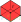
\includegraphics[width=0.8\textwidth, height=8cm]{figures/trivector.png}
   \caption{The trivector $\vec{\vec{e_1}} \wedge \vec{\vec{e_2}} \wedge \vec{\vec{e_3}}$ is the unit volume of 3D space, referred to as the pseudoscalar. The volume orientation is omitted in the figure for simplicity.}
   \label{fig:trivector}
\end{figure}
   


\subsection{The Geometric Product}

At the core of any algebra is an operation akin to multiplication. In linear algebra, we multiply matrices via specific rules. For elements in a GA, the rule is simple. For any two vectors $\vec{u}$ and $\vec{v}$, their geometric product is defined as
\begin{equation}
    \large \boxed{\vec{u} \vec{v} = \vec{u} \cdot \vec{v} \ + \vec{u} \ \wedge  \ \vec{v} },
\end{equation}
where $\vec{u} \cdot \vec{v}$ resembles the dot product, but I shall call it the inner product from now on. This terminology does not alter the mathematics in a strict sense at least for now, and the reader should interpret this term in the usual sense. Namely, the inner product of two vectors is a scalar--a measure of how two vectors are aligned in space, scaled by their lengths. Thus, the inner product term produces a grade-0 object in this case. 
\\ \\
The geometric product could be slightly unnerving at first glance, given the indoctrination of linear algebra typical of any physicist. However, we can interpret it using an analogy with complex numbers. Much like we add the complex numbers: 
$$ (a + ib) + (c -id) = (a+c) + (b-d)i , $$
one can think of same-grade components in a multi-vector adding together. Apples add with apples and oranges with oranges.
\\ \\
We need not contend too much with this idea for the moment, since, most of the time the geometric product reduces to either the inner or outer product term. As an example, consider the orthonormal basis for $\mathbb{R}^2$, $\{ \vec{e_1}, \vec{e_2}\}$. The product 
\begin{equation}
   \vec{\vec{e_1}} \vec{\vec{e_2}} = \vec{\vec{e_1}} \wedge \vec{\vec{e_2}},  
\end{equation}
because $\vec{\vec{e_1}} \cdot \vec{\vec{e_2}} = 0$, since the basis vectors are orthogonal. This applies to any of the basis vectors. On the other hand,
\begin{equation}
   \vec{\vec{e_1}} \vec{\vec{e_1}} = \vec{\vec{e_1}} \cdot \vec{\vec{e_1}} = 1, 
\end{equation}
since the area $ \vec{e_1} \wedge \vec{e_1}$ vanishes and the basis vectors are normalized. This simplification scheme will be our bread and butter in what is to come.